%\documentclass[a4paper,10pt]{article}
\documentclass[twoside]{iitbreport}
\usepackage[utf8]{inputenc}
\usepackage{graphicx}
\usepackage{natbib}
\usepackage{listings}
\usepackage{multicol}
%\usepackage[hidelinks]{hyperref}
\usepackage{xcolor}
\usepackage{comment}
\usepackage{enumerate}
\hypersetup{
    hidelinks,
     colorlinks,
    linkcolor={blue!30!black},
    citecolor={blue!50!black},
    urlcolor={blue!80!black}
}

\setcounter{secnumdepth}{4}
\setcounter{tocdepth}{4}
\degree{M.Tech}
\dept{Computer Science and Engineering}
\monthyear{OCTOBER 2016}
%opening
%\title{//TODO: write topic - "user space driver installation in LXC containers" , "bridging gap between VMs and containers"}
\title{Bridging the gap between virtual machines, and containers}
\author{Sahil Singh\\ (Roll Number 143050001) \\ {\normalfont under the guidance of} \\ Prof. Purushottam Kulkarni}

\begin{document}
 \let\cleardoublepage\clearpage
\maketitle

\begin{abstract}\thispagestyle{empty}
Linux Containers offer a more efficient manner of virtualizing user-space applications, as compared to virtual machines. This efficiency comes at the cost, and in many ways the former are less capable than the latter. One such way is the allowance of access to the kernel by installation of a kernel module. A shared kernel precludes any possibility of giving any one container access to it without worrying about isolation. An important question which arises then is, can there be a solution which maintains the efficiency of containers, while providing the isolation offered by virtual machines? This work tries to find a middle ground between the two, and introduces an implementation, using which a class of kernel modules can be allowed to be installed from the containers.
\end{abstract}
\newpage
\tableofcontents
\newpage
\let\LaTeXStandardClearpage\clearpage
\let\clearpage\relax
\listoftables
\listoffigures
\let\clearpage\LaTeXStandardClearpage
\newpage
\chapter{Introduction}
\begin{comment}
Traditional operating systems divide the code running on the system into two broad privilege levels\footnote{This doesn't mean that the hardware doesn't support additional privilege levels. Intel x86 comes with the so called 4 rings of operation, in addition to the SMM(System management mode). VT-x on this architecture introduces 2 new modes of operation - Root, and non-root mode.}. These are called the system mode, and the user mode. The system mode is the higher privilege mode of the two. The code which is critical for system functionality of the whole system, unsurprisingly resides in the system mode. This mode is the arbiter of all the resources in a system, and provides interfaces which can be used by the lower privilege mode, the user mode to access, and consume system resources. The user mode contains application programs  
which are used by people to carry out their daily tasks. Since, this is the lower privilege mode, it has lesser impact on the stability of the system. For instance we may never see the system crashing because of a misbehaving word processor, while a rogue driver, running in the system mode can easily bring the system down. This work is concerned with the x86 architecture, therefore the terms ring0, kernel mode, kernel space, and system mode may be used interchangeably. Similarly user mode, user space, and ring4 can be used in synonymously.
\end{comment}

Linux containers\footnote{Here the term is used in a generic sense, and not specifically for LXC} refer to a class of techniques used to group user space processes into isolated, and restricted domains. Unlike conventional virtualization techniques, the kernel is shared across the domains. This leads to lower resource consumption (memory, and CPU), and makes the solution very efficient. Since, the kernel is shared, there are several usage scenarios where we can use conventional virtualization techniques, but not containers. These are the scenarios where access to the kernel mode is required.

Let us consider an example. The CRORC(Common Read Out Receiver Card, figure~\ref{fig:crorc_card1})\footnote{http://www.cerntech.hu/products/5-crorc.html} card is used for collecting of data from an ongoing experiment at CERN\footnote{European Organization for Nuclear Research} over optic fiber cables. Its driver is mostly written in user space, with a small kernel space stub. If the user decides to run the application which gathers data from this card in a container, at the same time using another container for processing the data, while there are several other containers from different users running on the same underlying hardware, it cannot be done. If we instead use virtual machines(VMs) for this, the task becomes trivial. The user will just have to pass-through the card to the correct VM, inside which its driver can be run. Trying to do this in containerized  environment will be frowned upon, since the driver will get access to the whole kernel(remember that in case of containers, the kernel is shared), and may interfere with containers of other users.

\begin{figure}[ht]
\centering
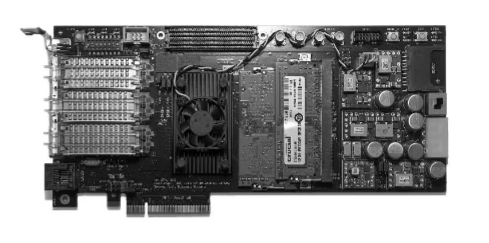
\includegraphics[width=375px]{crorc-card}
\caption{CRORC (Common Read Out Receiver Card), source:\cite{Eschweiler2014TheArchitecture} \label{fig:crorc_card1}}
\end{figure}


\section{Virtual machines and containers}
There are several subtle differences between the two, which requires a high level comparison.

A VM offers the following advantages.
\begin{itemize}
\item Isolation and Security

The whole operating system, along with application programs are made to run in isolated environments. If one VM gets affected by a security threat, it will not pose as great a risk, as in case of containers, since the kernel is shared.
\item Access to kernel space

This gives more flexibility to the user, in terms of the applications that can be developed. Some of the use cases which require access to the kernel are following.
\begin{itemize}
\item Using custom TCP/IP stack, new network protocols, etc.
\item Special devices
\item Different process schedulers
\item WSS estimate

\end{itemize}
\item Multiple OS support

Virtual machines provide an abstraction of a bare metal machine, on top of which one can install any software of his or her choice, including the choice of operating systems.
\end{itemize}
A container on the other hand offers the following advantages.
\begin{itemize}
\item Low resource consumption.

The kernel is shared, hence spawning a new container is as simple as creating few new processes, which is much lighter on RAM and CPU, as compared to booting a complete OS. The network, and disk I/O overheads are also less, as compared to a VM where these are emulated.

\item Small start-up time.\\\\
\end{itemize}

Having done a brief high-level comparison of the two, a question which arises is that, is there a middle ground between the two? In other words, will users always have to choose between efficiency, and flexibility?
This work tries to find a middle ground between the two, by allowing a class of drivers to be installed in the kernel from one container without compromising other containers running on the system, namely the user space drivers.
User space drivers are a class of device drivers, which have their majority of code written in the user space, with a small kernel stub. This kernel stub is necessary to handle interrupts in a reliable and efficient way. Since, the kernel space code is minimal, it only requires few services from the kernel.

By using virtualization extensions provided by a modern x86 processor, a separate and isolated execution context can be created in which these drivers can be made to run. There are several aspects of the problem that has to be consider, before a solution can be written. For example, handling of interrupts, communication of the driver with the processes in the container, etc. are just a few of them. These are expounded in the design and implementation sections.

\section{Problem statement\label{sec:problemstatement1}}

Allowing containers to install the kernel stub of user space drivers, subject to the following constraints.

\begin{enumerate}[(i)]
\item There is one to one mapping between a device and a container, i.e. the device for which driver is being installed is not multiplexed between several containers.
\item The kernel stub requires no kernel service, other than to register for and handle interrupts, to interact with the user space of the container, and memory management.
\item The device, and the CPU support pass-through. 
\item The CPU supports Interrupt remapping\footnote{https://pve.proxmox.com/wiki/Pci\_passthrough\#IOMMU\_interrupt\_remapping}.
\item The user should not be required to change the module for the user space driver in any way, neither should the source code of module be required.
\end{enumerate}

Allowing containers to install the kernel stub of the user space drivers will allow the driver to function completely, since the user space part is not  restricted in any way. 

Having defined, the problem statement precisely, we will establish the significance of the problem in section~\ref{sec:motivations}. We will then move onto the design and implementation where we will try to understand the reasons behind selecting user space drivers, after learning about some of the technologies used in this work.

\section{Motivations for giving containers an access to kernel space \label{sec:motivations}}
Giving containers access to the kernel started from the point of view of pure scientific research. This however, doesn't mean that it has no real world applications. This section tries to establish real world importance of the work, both in the context of User space drivers, and in general.

\begin{itemize}
\item Linux kernel has \textbf{UIO}. In Linux kernel, a new feature is allowed only if it has strong real world applications. This implies that the User space drivers form an important type of drivers in Linux. There are several areas where user space drivers are extensively used, particularly in scientific research for supporting specialized hardware. 
\item With the upcoming support of SRIOV and MRIOV in the hardware, the user space drivers can be used to allow individual containers to use the devices in any way it wants.
\item \textbf{Checkpoint/restore}\\
Giving containers ability to freeze, create checkpoints, restore, migrating processes into and out of containers.
\item \textbf{Custom driver for devices}\\
The container may choose to use a different, perhaps more optimized version for a device that it is using.
\end{itemize}

%\chapter{Exploring the design space\label{ch:designSpace}}
%For bridging the gap between a VM, and the container, the solutions can come from either side of the bridge. The VMs can be engineered to offer the efficiency of containers, conversely the containers can be made to support the flexibility of the VMs.

\chapter{Related work}
\textbf{ELKVM}\cite{pester2014elk} is a library using which an x86 elf executable can be run in an isolated space created by virtualization extensions. It was developed to intercept and analyze the system calls being made by an application. It creates an address space similar to Linux, however in place of actual kernel a proxy os resides, which does the task of forwarding the system calls to the host. On a system call made by an application, it saves information about the call, and issues a \textit{vmcall} to the host. A program running in host analyses the data stored by proxy OS to determine the details of the system call.\\

\textbf{ELK Herder}\cite{pester2014elk} is a software framework which is built on top of ELKVM. It runs an application in triple modulo redundant way to provide fault tolerance and recovery on off the shelf systems. It uses system calls made by an application as points of synchronization for the replicas. So, if replica 1 makes a system call A, it will wait for other two replicas to make the system call. When all 3 replicas reach this point of making call A, it checks the arguments of system call for all 3 replicas. If they are same, it implies no fault, else the arguments for which 2 of the 3 replicas agree are taken as correct. The replica which differed is considered faulty, and is discarded. In place of the discarded replica, a new replica is created by cloning one of the correct replicas.\\\\

\textbf{Arrakis}\cite{186140} reduces network overhead by bypassing the kernel and delivering packets directly to the user space. Each application has its own network stack. To multiplex the access to the network card, Arrakis relies on SRIOV.
\\\\
Apart from these, there are several other projects which take advantage of moving to user space, processing which has traditionally been limited to the kernel. These are discussed in chapter~\ref{ch:usduio}.
\\\\
This work differs from ELKVM and ELK Herder in the fact that while they were concerned in running a user space application in an isolated space created using virtualization extensions, this work is concerned with running a kernel module being installed from a container.

%\chapter{Virtualization}
%\section{Virtualization extensions}
%\subsection{KVM API}

\chapter{Linux containers}
Linux containers is an operating system level virtualization technique. It uses various mechanisms provided by the OS to isolate a group of processes, and control their resource allocation. LXC is one implementation of the technique. It relies on 3 Linux mechanisms.

\begin{enumerate}
\item Capabilities
\item Namespaces
\item Cgroups
\end{enumerate}

\section{Capabilities}
Traditionally, for security, the processes in an OS were distinguished into two.

\begin{enumerate}
\item Privileged
\item Unprivileged
\end{enumerate}

Privilege processes have super user rights on the system, while unprivileged processes have limited rights. Starting with Linux 2.2 the privileges of a super user are divided into several units. These are known as capabilities. Some of them are:

\begin{itemize}
\item \textbf{CAP\_SYS\_MODULE}\\
This capability allows installation of kernel modules. A process lacking this capability, even if it has user id 0 (root) will not be able to install a kernel module.

\item \textbf{CAP\_NET\_ADMIN}\\
This allows a process to do various network related operations like modifying IP tables.

\item \textbf{CAP\_NET\_RAW}\\
A process having this capability can create RAW and PACKET sockets. For example, if we have a program called \textit{hello\_raw} which creates a raw socket. If we run the program ,we will get permission denied error. However, if we give it textit{CAP\_NET\_RAW}, it will run successfully.\\
\begin{lstlisting}
gcc hello_raw.c -o hello_raw
./hello_raw
ERROR: Operation not permitted

sudo setcap cap_net_raw=ep hello_raw
./hello_raw
SUCCESS
\end{lstlisting}
\end{itemize}

Each process has three capability sets associated with it.
\begin{enumerate}
\item \textbf{Effective}\\
The capabilities that a process at a given time.
\item \textbf{Permitted}\\
The capabilities that a process can have throughout its lifetime. This is a super set of effective and Inheritable sets.
\item \textbf{Inheritable}\\
This set represents the capabilities that a process can pass to a child.
\end{enumerate}

The file corresponding to a process also has these three sets. See the previous example where we assigned capability to a file.

The net effect of these group of sets (capability sets of file and capability sets of a process in execution) is that a process always has the lower capabilities when both types of capability sets are compared.

\section{Namespaces}
Namespaces provide a mechanism to isolate a system resource in a way that a processes in a particular namespace feels as if they have their own instance of that resource. For better understanding let us consider an example.\\
Suppose we have two bash shells open on our system, bash1, and bash2. A "\#" indicates a comment. Every row in the following output corresponds to the same time instance, thus if command is entered in bash1, but not in bash2, then the $2^{nd}$ column of that row will just show the bash2 prompt.\\

\begin{multicols}{2}
\begin{lstlisting}
bash1$>ls /mnt
bash1$>
#/mnt is empty
bash1$>ls /tmp
A B C D
#contents
#of /tmp
bash1$>sudo unshare -m bash1
#create new mount 
#namespace 
#with unshare command
bash1#>
bash1#>mount --bind /tmp /mnt
bash1#>
bash1#>ls /mnt
A B C D
#/mnt NOT empty
\end{lstlisting}
\columnbreak
\begin{lstlisting}
bash2$>ls /mnt
bash2$>
#/mnt is empty
bash2$>ls /tmp
A B C D
#contents
#of /tmp
bash2$>
#
#
#
bash2$>
bash2$>
bash2$>
bash2$>ls /mnt
bash2$>
#/mnt empty
\end{lstlisting}
\end{multicols}

Linux currently has 6 namespaces. This may change in future, as new namespaces are proposed, or old ones need removal.

\begin{enumerate}
\item \textbf{Mount Namespace}\\
Isolates file system mount points, as we saw in the previous example.
\item \textbf{UTS Namespace}\\
Isolate the two system identifiers - node name, and domain name.
\item \textbf{IPC Namespace}\\
Isolate IPC\footnote{Inter Process Communication} resources
\item \textbf{PID Namespace}\\
Isolate PID\footnote{Process Identifier} number space. Processes in two different PID namespaces can have the same PID with respect to their namespaces.
\item \textbf{Network Namespace}\\
Isolate networking resources, such as network device, routing table, etc.
\item \textbf{User namespace}\\
Isolate user and group ID number spaces. A process's user and group ID can be different inside and outside a user namespace.
\end{enumerate}

\section{Cgroups}
Cgroups is a mechanism to limit, and account the usage of resources(such as memory, CPU, etc.) by a group of processes. Using Namesapces along with Cgroups, we can see that a VM like domain can be created in which the processes see the resources allowed by namespaces, and use them upto a limit specified by Crgoups. For example using Namespace a groups of processes can be created which will feel that they are the only processes running on the system, and using Cgroups they can be allotted say 500MB of ram. This is the underlying idea of containers.

\section{Confluence of Capabilities and Namespaces}
Linux capabilities were introduced in kernel 2.2, while Namespaces in kernel 3.8. Two technologies separated so far apart in the release cycle came to a confluence in a patchset proposed by a kernel developer Serge E. Hallyn\footnote{http://www.kernelhub.org/?p=7\&dev=2755\&mbox\_type=5}. The patchsets enabled the use of Capabilities and Namespaces together. Let us first revisit the two, in order to understand how they work together.
\\
\textbf{Linux Capabilities}\\
These came into picture to fine grain the power of root (EUID 0, traditionally the programs running with SUDO). Before that a program running as root was all powerful. Now let's say I am running wireshark, it should only have network related powers, and if it tries to insert a kernel module (say someone exploited my wireshark instance) it should be denied. With just EUID being a check of powers, it was not possible. Now I can give wireshark the ``CAP\_NET\_ADMIN" and ``CAP\_NET\_RAW" capabilities (and perhaps some others which are related to networking), and not give ``CAP\_SYS\_MODULE".\\

\textbf{User Namespace}\\
User Namespaces isolate security-related identifiers and attributes, in particular, user IDs and group IDs, the root directory, keys, and capabilities. A process's user and group IDs can be different inside and outside a user namespace. In particular, a process can have a normal unprivileged user ID outside a user namespace while at the same time having a user ID of 0 inside the namespace; in other words, the process has full privileges for operations inside the user namespace, but is unprivileged for operations outside the namespace. \footnote{source : man page (http://man7.org/linux/man-pages/man7/user\_namespaces.7.html)}\\
The following line from Wikipedia sheds some light.\\
``Permissions for namespace of the other kinds are checked in the user namespace, they got created in.'' \footnote{source : wikipedia (https://en.wikipedia.org/wiki/Linux\_namespaces)}.\\

So in a way user namespaces, like user and group IDs in a traditional system control the access to various components of it (for example, managing files, killing processes, etc.). The only thing different in case of user namespaces is that the ``system" is defined by other parameters related to it, like the mount namespace, PID namespace, etc.

The line above from Wikipedia then says that if a process in user namespace UN1 has the capability to kill other processes, and if it tries to kill a process in another user namespace, say UN2, where UN1 and UN2 are disjoint, and one is not the ancestor of other, then this must not be allowed.

\textbf{The confluence}\\
The intersection of the two technologies allow an unprivileged process to create new user namespace , where it has full capabilities. Thus in the ``pseudo system" created by it, it will be able to use Linux capabilities, but outside this ``system", it will be powerless. By ``pseudo system" I mean creation of a new user namespace, and assigning of resources to it using other namespaces like PID, mount, net, etc.\\
If we have a look at all the places in the Linux kernel where the checks of capability is being made, we will see two types of checks, depending on the operation that is being performed.

\begin{enumerate}
\item Checks with respect to user Namespace of the process\\
For operations in which one process tries to affect another process, it is important to check that the process trying to affect another process has the required Capabilities in the user Namespace of the other process. For example if one process is trying to kill another process, it must have ``CAP\_KILL" in the user Namespace of the process it is trying to kill.

\item Checks that consider the capability with respect to the \textit{init\_user} Namespace\\ (\textit{init\_user\_ns})\footnote{init\_user\_ns is simply the root user namespace, i.e. the user namespace that is created at boot time.}.\\
There are some actions which have system wide consequences, for example if a process P1 tries to install a module. Such checks are made with respect to the \textit{init\_user} Namespace. There is no meaning to the question, ``is this user allowed to install module with respect to his or her own namespace?", since the installation will affect the whole system. Thus a better question to ask would be, `Is this user allowed to install module with respect to the root namespace (\textit{init\_user}) ?". Since, the \textit{init\_user} will anyway be ancestor of all other namespaces, thus it will have a system wide scope.	
\end{enumerate}

\chapter{User space device drivers and UIO\label{ch:usduio}}
Figure~\ref{fig:user-space-driver1} shows the architecture of a user space driver. A user space driver has two parts.
\begin{itemize}
\item Kernel module
\item User space application program
\end{itemize}

As can be inferred from the name, the bulk of driver logic resides in the application program running in the user space. The kernel module has a small amount of code, which couldn't be written in user space, or would have been very difficult.

\textbf{Kernel module} of the user space driver registers itself with the driver subsystem. This causes the driver to be probed, when a device supported by the driver is attached to the system. It also is responsible for handling interrupts from the device. A user space interrupt handler cannot be used because of the following two reasons. 

\begin{itemize}
\item A user space application may crash, taking down the interrupt handler with it. Thus a kernel space interrupt handler makes the driver more robust.
\item The latency of handling interrupts will be more, since we may have to wait for the process to schedule back in, if it is not running at the time the interrupt gets delivered.
\end{itemize}

The module exposes several files in the user space in the form of \textit{/dev}, \textit{/proc}, or \textit{/sys} entries. Using which the user space part can communicate with it. Using these files, the user space can also \textit{mmap} memory regions of the device, and access information about interrupts.

\textbf{User space application program} talks to the device via the kernel module. The information about the memory regions of the device is obtained by it using \textit{/sys} entries exposed by kernel module. It then does an \textit{mmap} on each of the region. This allows the user space part of the driver to directly access the memory of the device. The interrupts however have to be channeled through the kernel module. The mechanism of interrupt delivery to the user space is the following.

\begin{itemize}
\item Application does a \textit{select()} system call on a file exposed by the kernel module (typically a \textit{/dev} entry).
\item When an interrupt occurs, the kernel module acknowledges it, and writes an entry in the corresponding file exposed to the user space.
\item This write causes the user space program to wake up, which then takes a suitable action.
\end{itemize}

There are several reasons for preferring a user space application over. This does not mean however that a user space driver should always be preferred over a kernel space driver. The following are the advantages, and limitations of the user space drivers.

\begin{figure}[ht]
\centering
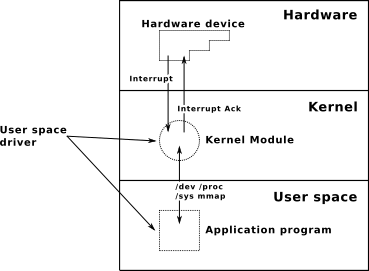
\includegraphics[width=375px]{user-space-driver1_svg}
\caption{Architecture of a user space driver\label{fig:user-space-driver1}}
\end{figure}

\section{Advantages of user space drivers}
\begin{itemize}
\item The user space API of the kernel is kept stable to prevent breaking of applications. The in-kernel API however keeps on changing. Any application developed in user space is guaranteed to work for long.
\item Bugs in the user space part of the driver will not crash the kernel. Since in case of user space drivers, the majority of code lies in the user space, it will be safe to assume, that the changes of finding a bug there are higher. This becomes even more important when we consider the fact that 70\% of the code of Linux kernel comprises of drivers, and the majority of bugs of the kernel are contributed by them\cite{Chou2001AnErrors}.
\item There are a large number of tools available for developing and debugging user space applications. Specially debugging a user space application is much easier than debugging any piece of kernel space code.
\item Floating point operations can be done in user space.
\item The user space is rich in the number of available libraries and frameworks. The user space driver may even be developed in python.
\end{itemize}

\section{Limitations of user space drivers}
\begin{itemize}
\item Doesn't completely eliminate the need for a part of the driver to run in the kernel space.
\item Interrupt handling isn't  efficient.
\item Performance is poor as compared to a purely in-kernel device driver.
\\\\The previous two points are argued against in the paper \textit{ The Portable Driver Architecture}\cite{Eschweiler2014TheArchitecture}. However the debate is still open regarding their performance and efficiency.
\item While the kernel code is required to be GPL license compatible, there is no such restriction on user space code. This may encourage proliferation
of closed source binary-only drivers. This will harm the open source movement, and also the quality of code being produced.
\item Multiplexing of user space drivers isn't easy. If the driver has to be accessed from multiple processes, a kernel space driver will suit better\cite{userSpaceDriversTldp}\cite{xilinxUIO}. 
\item There is no predefined API for other user space applications to get access to user space drivers.
\item Certain kernel frameworks like DMA, direct cache control, contiguous memory allocation, etc. are not available directly to user space.
\end{itemize}

\section{Use cases}
\begin{itemize}
\item When working with a new and unusual hardware, user-space drivers can be used for initial understanding, without risking the stability of the entire system.
\item Hardware that doesn't fit into one of the kernel subsystems like fieldbus cards, industrial I/O cards, A/D converters, custom FPGAs, etc. are generally used and developed by engineers who are not kernel experts, thus writing code in user space will be beneficial for them.
\item The internal API of kernel changes frequently. The drivers that are mainlined into the Linux source are maintained by the community. Thus, when a part of kernel changes, the affected drivers generally are taken care of by the developer making the change. It is difficult to get the code for some special hard ware mainlined, therefore maintaining it over different kernel versions will be difficult.


\end{itemize}
\section{UIO}
The user space device driver architecture that we have seen till now is a generic term encompassing a variety of techniques, which are used to allow bulk of driver code run in the user space. Different developers have tried different approaches for this, and there has been different mechanisms of supporting such drivers in the Linux kernel. The underlying principles remain the same as the ones discussed above.\\
\\
The term UIO, which stands for user space I/O is the support offered by the kernel nowadays. It makes the task of developing a user space driver even simpler. It exposes a character device in the user space which can be used by the user space part of the driver. It also creates file attributes in \textit{/sys} describing the attributes of the device. These attributes are nested in \textit{/sys/class/uio}. The kernel space component is still required for most user space drivers, but now its development becomes even simpler. The kernel component just has to register itself with UIO framework (called the UIO core), giving it information about the device, interrupt handler, etc. The UIO core then automatically creates user space entries. For every device attached, the UIO core creates a \textit{/dev/uioN} file, where N starts from 0, thus the first device will correspond to \textit{/dev/uio0}.

UIO core supports two kinds of device drivers.

\begin{enumerate}[(i)]
\item UIO device driver
\item UIO platform device driver
\end{enumerate}

The first term refers to all those device drivers that use UIO framework, but do not handle platform devices. Platform devices are devices like com ports, debug ports, etc. which are connected to the CPU directly\cite{deviceDriverArchitectureLinux}. These devices don't support enumeration, i.e. unlike other devices which can, these devices will not identify themselves automatically. The driver handling these devices should know their properties. For example if a driver handles a com port platform device, it must know the address, or port number of the CPU where it should write to. A USB device on the other hand would generally identify itself (There can be a platform USB device as well, in that case it will not identify itself). 
\\\\
User space drivers for platform devices don't require any kernel module to be written. The kernel space requirements are handled by the UIO core itself. There only has to be a user space component. The other kind of UIO drivers do require a kernel space module.
\\\\
\begin{figure}[ht]
\centering
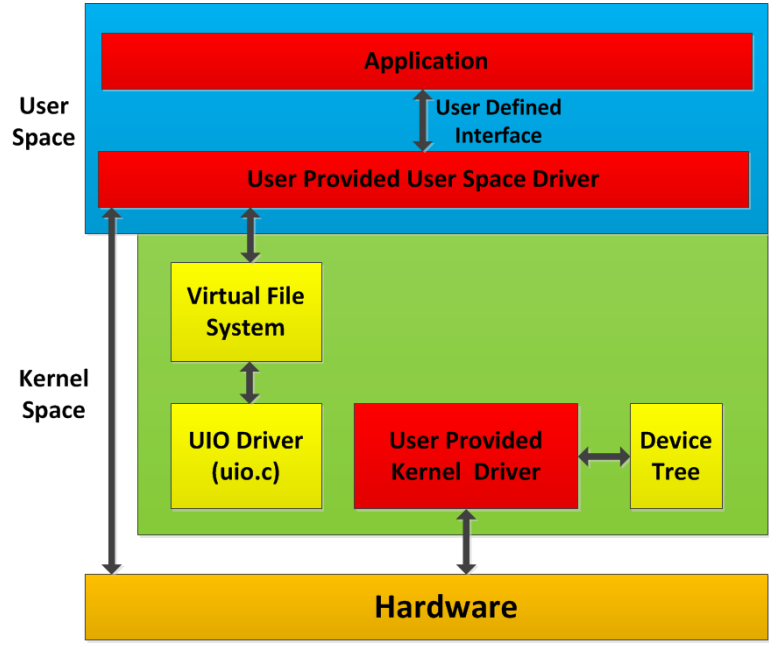
\includegraphics[width=375px]{uio-driver}
\caption{UIO driver (non-platform) \footnotesize{source:\cite{xilinxUIO}} \label{fig:uio-driver1}}
\end{figure}

\begin{figure}[ht]
\centering
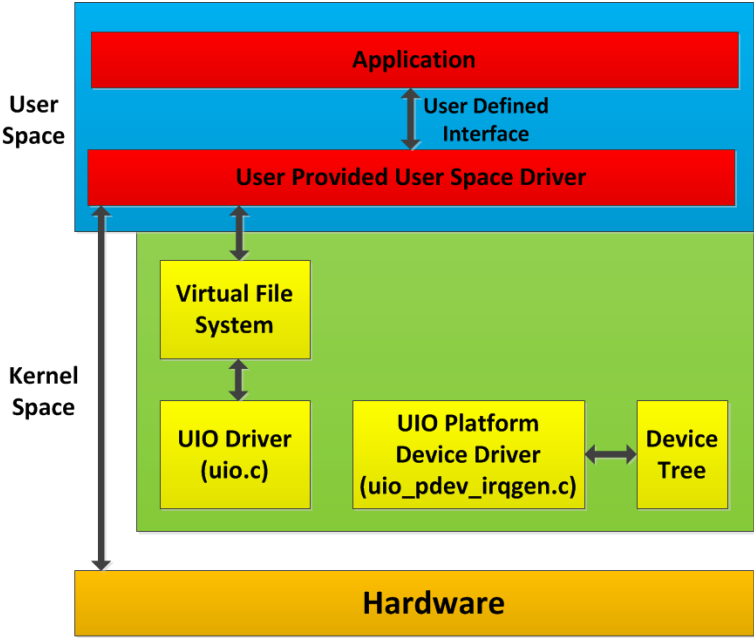
\includegraphics[width=375px]{uio-platform}
\caption{UIO platform driver \footnotesize{source:\cite{xilinxUIO}} \label{fig:uio-platform1}}
\end{figure}

Figure~\ref{fig:uio-driver1} and figure~\ref{fig:uio-platform1} show the architecture of the two. The block corresponding to \textit{uio.c} in both the figures correspond to UIO core. There are two things to notice in these figures.

\begin{enumerate}[(i)]
\item The interfaces between ``Application", and ``User Provided User Space Driver" are marked ``User Defined Interface". Contrast this to conventional device drivers running in kernel space which have a well defined interface.
\item In figure~\ref{fig:uio-driver1} there is a red box in the kernel space marked ``User provided Kernel Driver". This box is absent in figure~\ref{fig:uio-platform1}. This is as expected since, UIO platform drivers don't require a user provided kernel driver.
\end{enumerate}

\section{Userspace driver frameworks}
There are several other frameworks which either support development of user space drivers, or make use of them. We have already discussed UIO, here are some others.

\begin{enumerate}
\item \textbf{UIO}\\
This is supported in Linux kernel.
\item \textbf{Intel DPDK (Data Plane Development Kit)}\\
This is for x86 architecture.
\item \textbf{USDPAA (User-Space Data Plane Acceleration Architecture)}\\
This is for PowerPC and ARM.
\item \textbf{TransportNetLib}\\
This is for ARM's keystone architecture.
\item \textbf{Open Data Plane}\\
\end{enumerate}

The application of user space drivers for networking is also an active area of research. The following is a list of user space network stacks\footnote{Linux as well as non-Linux stacks}.

\begin{enumerate}
\item \textbf{Developed from scratch}\\
\begin{enumerate}
\item \textbf{mTCP}\cite{mTCP}\\
Highly scalable user space TCP stack for multi-core systems.
\item \textbf{Mirage-tcpip}\cite{mirage-tcpip}\\
Developed in OCAML language.
\item \textbf{lwIp}\cite{lwip}\\
Tiny TCP/IP stack that aims to reduce RAM footprint. 
\end{enumerate}
\item \textbf{Ported from existing stacks}\\
\begin{enumerate}
\item \textbf{Arrakis}\cite{arrakis}\\
Derived from lwIp.
\item \textbf{libuinet}\cite{libuinet}\\
Derived from freeBSD.
\item \textbf{NUSE}\cite{nuse}\\
A libOS implementation of Linux kernel.
\item \textbf{OpenDP}\cite{OpenDP}\\
Derived from freeBSD.
\item \textbf{OpenOnload}\cite{OpenOnload}\\
High performance user level network stack. Derived from lwIp.
\item \textbf{OSv}\cite{osv}\\
Derived from lwIp.
\end{enumerate}
\end{enumerate}

\chapter{Design}
In a containerized environment the kernel is shared among the containers. Thus if any one container gets access to the container, it can monopolize the entire system. The situation is shown in figure~\ref{fig:problem1}. In the figure notice that when module M1 is installed it gets unrestricted access to the system. \\
Container solutions prevent this from happening by using various security mechanisms. 
LXC in particular drops \textit{ sys\_module} capability\cite{capabilityInLinux26} when starting a container. This capability is required for installation of kernel modules. On top of that it also limits access to \textit{finit\_module},  \textit{init\_module}, and \textit{delete\_module} system calls using SECCOMP~\cite{seccomp12} filters. For example, in Ubuntu, the default filter for LXC containers is located in\\ \textit{/usr/share/lxc/config/common.seccomp}. \\
Here, are its contents on Ubuntu 16.04, running lxc 2.0.4.\\

\texttt{2\\
blacklist\\
reject\_force\_umount  \# comment this to allow umount -f;  not recommended
[all]\\
kexec\_load errno 1\\
open\_by\_handle\_at errno 1\\
init\_module errno 1\\
finit\_module errno 1\\
delete\_module errno 1
}
\\
\\
An ideal scenario which we would like to have is one in which even after allowing installation of kernel module, the module is limited to a finite set of kernel API it can access. It should also under no circumstances get access to other containers running on the system. This is shown in figure~\ref{fig:ideal1}.

\begin{figure}[ht]
\centering
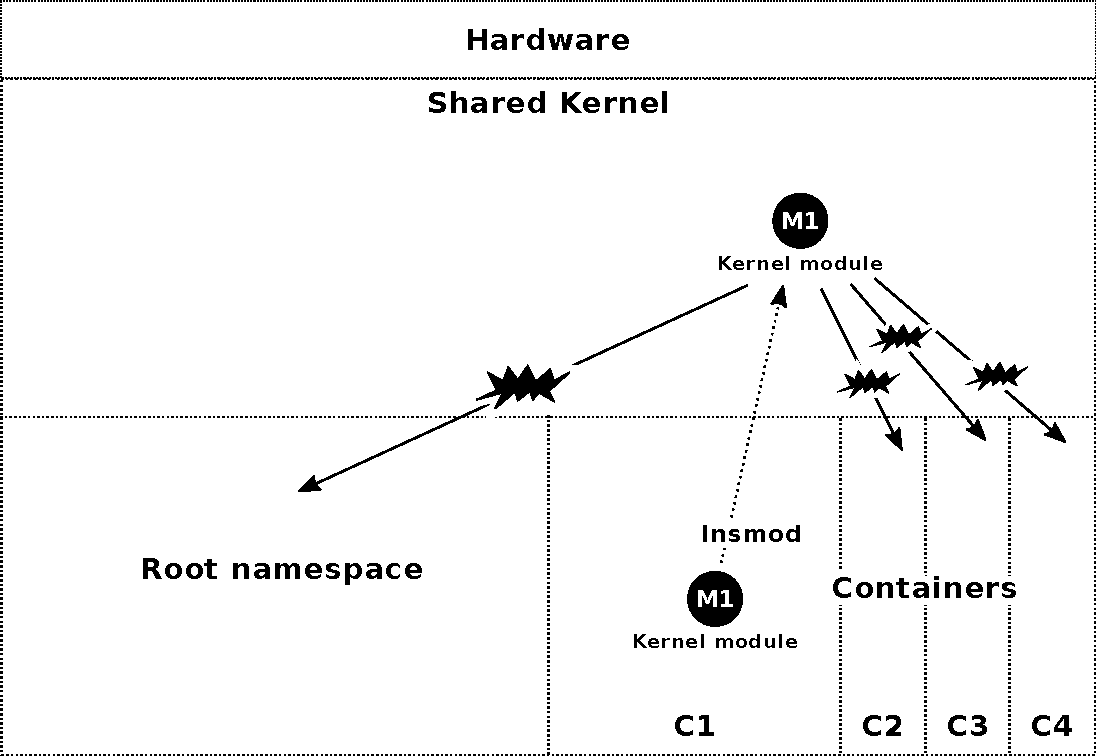
\includegraphics[width=\textwidth]{problem}
\caption{Allowing any container to install a kernel module will effectively give it an access to the entire system\label{fig:problem1}}
\end{figure}

\begin{figure}[ht]
\centering
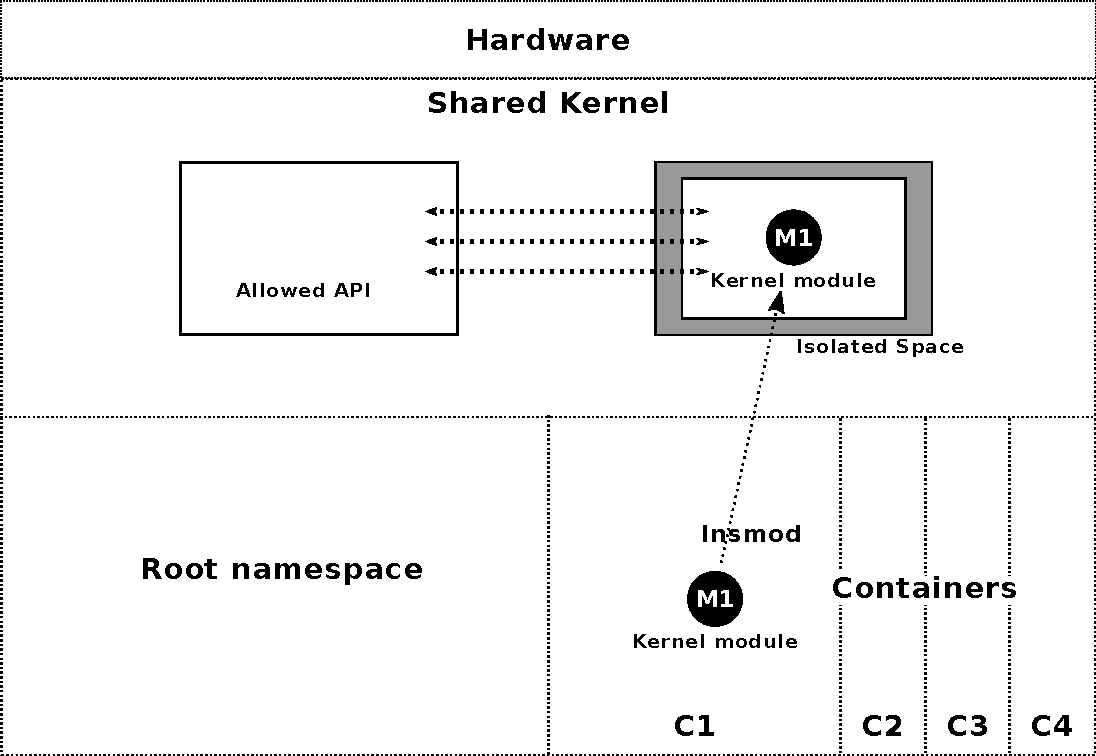
\includegraphics[width=\textwidth]{ideal}
\caption{Even after allowing the kernel module to get installed, it should have a limited access to the system.\label{fig:ideal1}}
\end{figure}

\section{Why user space drivers?}
We started off with an aim to find a middle ground between VMs and containers. We realized that the shared kernel is the main reason which gives efficiency to the containers, and also the main reason for its lack of flexibility when compared to VMs. We want to give containers an access to the kernel, without compromising the working of other containers. Allowing installation of kernel modules is one way in which we can give access to the kernel. Should we allow installation of each and every kernel module, even if it contains a halt instruction which just halts the machine, affecting other containers? The answer is obviously no. How then to decide which kernel modules are safe for installation, and which are not?

\subsection{Coupling and cohesion}
\textbf{Coupling}\footnote{https://en.wikipedia.org/wiki/Coupling\_(computer\_programming)} is the degree of interdependence between software modules; a measure of how closely connected two routines or modules are.

\textbf{Cohesion}\footnote{https://en.wikipedia.org/wiki/Cohesion\_(computer\_science)} refers to the degree to which the elements of a module belong together.
\\
\\
To keep a module in an isolated space when installed from a container, we would like to choose one which has low coupling with the kernel, and high cohesion. This will mean that at the beginning of our exploration to find the middle ground, we will have less things to worry about.


Here come the user space drivers. A user space driver, as already discussed has two parts, a kernel module, and a component running in the user space. Since, in the container the user space environment remains similar to an non-containerized system, the user space component should run equally well in a container as well. The kernel space component also has some suitable properties which makes it a nice candidate. It requires only a few functionality.

\begin{itemize}
\item Registering itself as a device driver
\item Handling interrupts from device
\item Memory management
\item A mechanism to talk to user space
\end{itemize}

This means very low and manageable coupling with the kernel.

\section{Overall design}
Let us revisit the problem statement (section~\ref{sec:problemstatement1}).
\\\\
\textbf{Problem statement}\\
Allowing containers to install the kernel stub of user space drivers, subject to the following constraints.

\begin{enumerate}[(i)]
\item There is one to one mapping between a device and a container, i.e. the device for which driver is being installed is not multiplexed between several containers.
\item The kernel stub requires no kernel service, other than to register for and handle interrupts, to interact with the user space of the container, and memory management.
\item The device, and the CPU support pass-through. 
\item The CPU supports Interrupt remapping\footnote{https://pve.proxmox.com/wiki/Pci\_passthrough\#IOMMU\_interrupt\_remapping}.
\item The user should not be required to change the module for the user space driver in any way, neither should the source code of module be required.
\end{enumerate}

We can see that constraints iii follows from i, and (iv) follows from both i and ii. We can create an environment for the kernel space component using virtualization extensions on modern CPUs.
\\\\
Figure~\ref{fig:overallDesign1} shows the overall design. The arcs labeled with numbers are the steps. They are the following.

\begin{enumerate}
\item \textbf{Insmod}\\
Container C1 installs kernel module. The kernel function \textit{load\_module()} is modified to check for installation of kernel modules from the containers. When it detects a module, it forwards the data representing module to the proxy module. Insmod now returns.
\item \textbf{Notify using eventfd}\\
The proxy module is responsible for copying the contents of the module in its tables, so that insmod can finish execution. The proxy module then notifies a server running in the root user space (outside of all containers) that a new module has come. Note that at this stage we do not have module's source code, we only have module's binary, along with relocation and symbol tables.
\item \textbf{Create isolated space}\\
The server creates an isolated space in which the module can be run.
It then tells the details of the isolated space to the proxy module, which then copies the module to this new space. Note that the task of copying the module could also be done by the server, but it is easier to do by the proxy module since copying of module to the user space is avoided, and the kernel already has functions and data structures which ease the copy.
\item \textbf{Copy and run the module}\\
The Proxy module then copies the module to the isolated space, and executes its \textit{init}\footnote{specified in the module's source code by module\_init() macro} function. \\\\
\end{enumerate}

Chapter~\ref{ch:implementation} elaborates these steps, going into details of each, and also does an in depth analysis of the whole process.

\begin{figure}[ht]
\centering
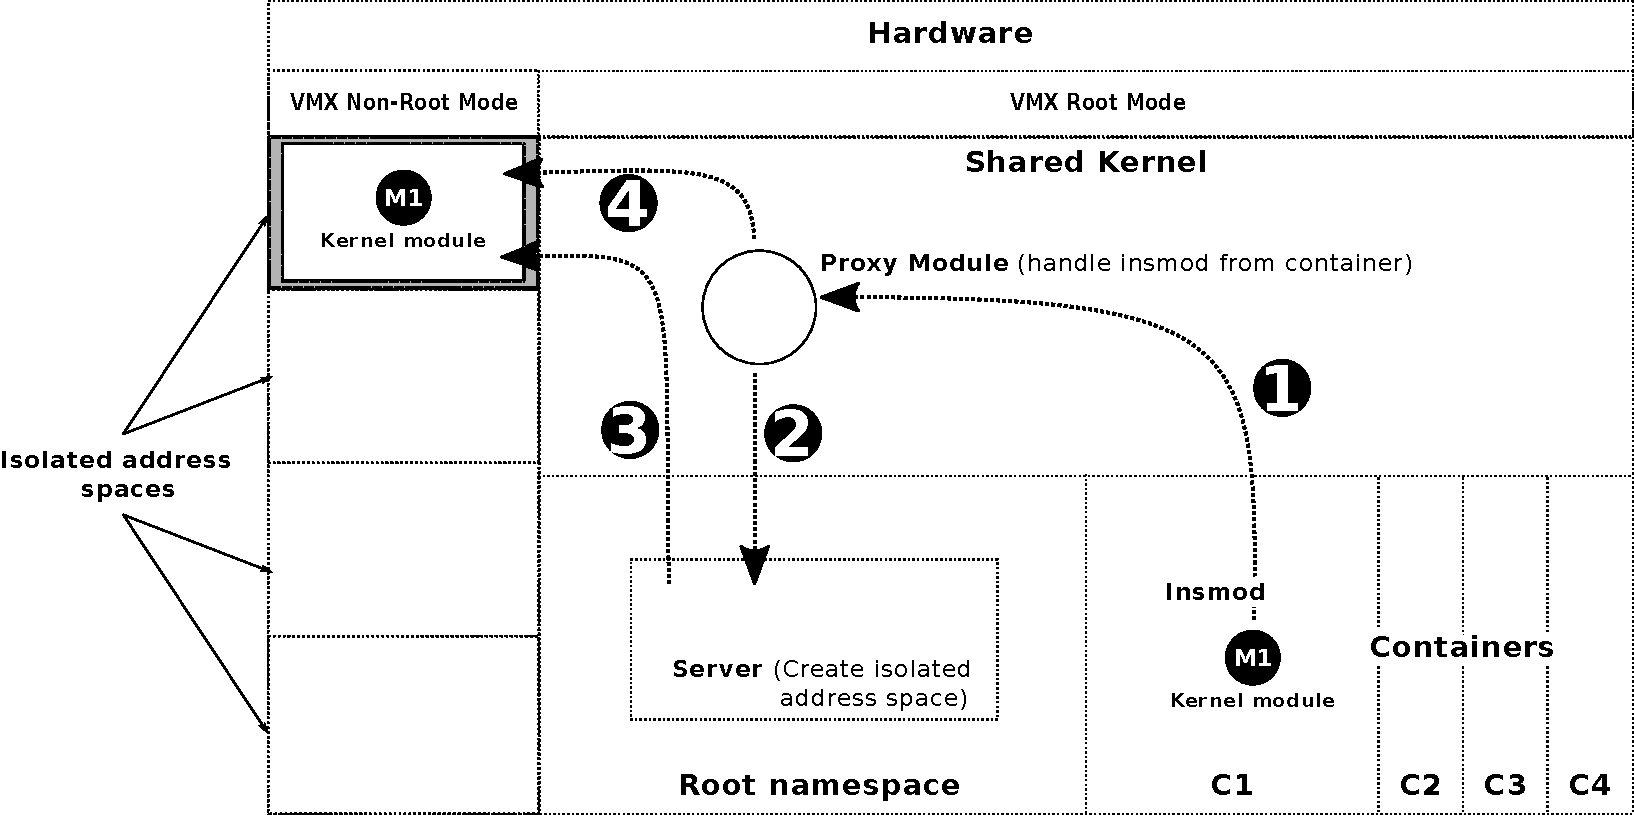
\includegraphics[width=\textwidth]{design}
\caption{Overall design\label{fig:overallDesign1}}
\end{figure}



\chapter{Implementation\label{ch:implementation}}
Figure~\ref{fig:componnts1} shows the main components of the project. These are explained as follows.

\begin{enumerate}
\item \textbf{Host server}\\
This is a server which runs inside the root namespace, i.e. outside of any containers. It uses KVM API to create an isolated space, where the module from the container gets loaded.
\item \textbf{Proxy module}\\
This component, aptly named as \textit{proxy module} is responsible for proxying data between the host server, the insmod program (which runs from within a container), and the isolated namespaces created for each module.
When insmod is being done from a container, a tap in the kernel function \textit{load\_module} sends the data corresponding to the module, which is in the form of an object \textit{struct module}, to the proxy module. This object contains the module binary and other meta data. If a Host server process has registered itself, the Proxy module sends a notification to it using eventfd, else it stores the object in an internal data structure, till a new Host server process registers itself. It is also responsible for copying module's binary correctly in the isolated space created by the Host server.
\\
Proxy module exposes the following two special files in the root namespace.
\begin{enumerate}
\item \textbf{/dev/lxc-uio-proxy}\\
This is the file used by Host sever for communicating with the Proxy module.
\item \textbf{/proc/lxc-uio-proxy-debug}\\
This is were the Proxy module writes the Major number the chardev (/dev/lxc-uio-proxy) got. This file is also use to view statistics about the internal table of modules maintained by the Proxy module, such as number of entries, current table size (table can dynamically grow), etc.
\end{enumerate}

\item \textbf{Insmod}\\
The installation of kernel module is limited in LXC by dropping \textit{sys\_module} capability when a container starts. Rather than preventing this drop\footnote{using lxc.keep or lxc.drop options in a container's configuration} we modify insmod, so that it sends an additional flag\footnote{MODULE\_INIT\_LXC} to the kernel, which tells the modified \textit{load\_module()} function in the kernel that this module is being installed from a container.
To send this flag the insmod program had to be modified. To send the modified flag using modified insmod, it must be invoked with ``-c" option. Note that both the option, and the flag are new, and are defined specially for this project.
\begin{lstlisting}
insmod -c hello_world.ko
\end{lstlisting}
\end{enumerate}



\begin{figure}[ht]
\centering
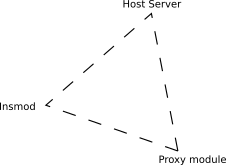
\includegraphics[width=0.5\textwidth]{components_svg}
\caption{Project components\label{fig:componnts1}}
\end{figure}

\begin{figure}[ht]
\centering

\includegraphics[width=0.85\textwidth]{tasks_svg}
\caption{Tasks to be performed\label{fig:tasks1}}
\end{figure}



These components together perform the following 10 tasks (figure~\ref{fig:tasks1}).

\begin{enumerate}
\item \textbf{Server registration}\\
When the server running in the root name space, called \textit{Host Server} (or as \textit{KVM Host Server} in some places) in the project, starts, it registers itself with the proxy module in the kernel.
The server first creates a file descriptor for event fd, and then makes an ioctl call to \textit{``/dev/lxc-uio-proxy"} to register itself. The integer value of eventfd file descriptor is sent as an argument with the ioctl.\\
When Proxy module receives this request, it stores the PID\footnote{Process ID} of the server, and the file struct corresponding to the eventfd file descriptor. This structure is used by the module to send notification to the Host server when a new module is installed.

\item \textbf{Module insertion}\\
Insertion of module from a container uses the modified insmod, as explained previously. On module insertion the kernel function \textit{load\_module()} allocates memory for the module, does its relocation and linking, and calls module's \textit{init}\footnote{specified in the module's source code by module\_init() macro} function. While all this is being done the modules state is \textit{MODULE\_STATE\_UNFORMED}. In the end, \textit{load\_module()} calls \textit{do\_init\_module()}, which sets module's state to\\ 
\textit{MODULE\_STATE\_LIVE}, and calls its \textit{init} function. As long as module's state is set to \textit{MODULE\_STATE\_UNFORMED} it will not be disturbed by any other part of the kernel. Its entry will exist in kernel's module list, but other than that it won't affect the system. Just before \textit{do\_init\_module()}, the module's code(which is relocated and linked by now) and meta data are stored in an object of type \textit{``struct module"}. Copying this object to the Proxy module is a better option than to rewrite code to apply relocations.\\
A tap inside the \textit{load\_module()} function checks if the module is being installed from a container. If it is, then call to \textit{do\_init\_module()} is prevented, and 0 (zero) is returned. This causes insmod to terminate successfully. The state of the module remains \textit{MODULE\_STATE\_UNFORMED}, and its \textit{init} function is not called. The \textit{init} function will be executed once the module is copied to the new isolated space created for it.
\\
The \textit{struct module} object of the module is copied to Proxy module. Since, at this point the module is present in kernel memory the pointers inside the object will remain correct.

\item \textbf{Notification}\\
When a new module is copied to the Proxy module, it sends a notification to the Host server, if one is registered, else it just stores the module until a server connects.\\
Eventfd is used for notifying the server instead of signals, since signals are delivered asynchronously to the main thread, and thus will introduce concurrency issues. The check of any event in server is done using the \textit{select()} system call in its main thread. Thus the execution of server remains single threaded. One thing to note is that when an eventfd event occurs, a read must be performed on its file descriptor to read its 64bit counter value, even if the value is not required. Unless this is done, the eventfd event will not reset, and the \textit{select()} system call will keep showing that new event has occurred, even if only a single event occurred initially.

\item \textbf{Isolated space creation}\\
An isolated space is created by utilizing virtualization extensions present on modern CPU. An execution environment is created in VT-x non-root mode. The module is then copied to it.\\
The characteristics of the isolated space are:\\
\begin{enumerate}
\item It has a separate address space than the host kernel, therefore it cannot access the kernel directly.
\item It runs in VMX-non root mode, while the host kernel and the containers run in VMX-root mode. Therefore, if it wants to access anything outside the space, a trap will be generated, and will be handled in host, which may then choose to do some emulation.
\item Different modules go to different isolated spaces. Therefore modules from one container cannot affect modules from another container. This however also prevents two modules from the same container from sharing things. This can be overcome in the next iteration of design.
\end{enumerate}

The virtualization extensions are made use of by using KVM API\cite{kvmApiDoc}. Here are the steps required(as shown in figure~\ref{fig:kvmHellowFlowchart1}).

\begin{enumerate}
\item \textbf{KVM\_fd=open(/dev/kvm, ...)}\\
Open a handle(file descriptor) to \textit{/dev/kvm} character device exposed by kvm.
\item \textbf{VM\_fd=ioctl(KVM\_fd, ...)}\\
KVM calls every execution context that we create a VM, in this work the execution context is called an isolated space, but VM may be used as well. A VM in some sense represents a virtual hardware. To it we then attach CPU, memory, etc. as per our liking. This \textit{ioctl} creates a VM, and returns a file descriptor for it.
When we will later attach memory, cpu, etc. to the isolated space, we will use this file descriptor.
\item \textbf{void * mem=malloc() or mmap()}\\
The VMs created by KVM use the memory of the host process issuing these calls. Thus to give memory to the VM, we must first allocate it for the process.
\item \textbf{Copy data/code to mem}\\
The memory allocated in previous step will form a part of the VM, we can therefore write the desired code and data, which in our case will be code and data of the kernel module to it. This will be the initial state of RAM for the VM we are creating.
\item \textbf{attach memory(mem) to VM}\\
This step associates the memory with the VM's file descriptor. While attaching we have to specify the region in guest's physical address space where this memory will be visible. For example if after \textit{malloc()} the memory region allocated points to 0x4000, we may then tell kvm that this memory should appear in guest's physical address space at 0x1000.
\item \textbf{VCPU\_fd=ioctl(VM\_fd, ... )}\\
This step attaches a single VCPU to the VM. Right now the isolated spaces get only a single VCPU, to keep things simple. Moreover there was no need felt to give multiple VCPUs.
\item \textbf{Set initial VCPU register values}\\
Set initial values of VCPU registers, such as instruction pointer, code segment register, etc.
\item \textbf{KVM\_RUN}\\
Now the VM (isolated space) is ready to run. The \textbf{init} function of the module should execute now.
\item \textbf{Handle exits}\\
During the course of execution the VM may exit several times, for example to do I/O. These have to be handled, and if required any emulation has to be done. After this VM is run again, or halt-ed if execution of module's \textit{init} function finished.
\end{enumerate}

\begin{figure}[ht]
\centering
\includegraphics[width=0.75\textwidth]{kvm-hello-flowchart_svg}
\caption{Steps for creation of an isolated space \label{fig:kvmHellowFlowchart1}}
\end{figure}


\item \textbf{Linking and relocation}\\
When a module is compiled, it lacks the symbols exported by the kernel. While installing the module the references to these symbols have to be made to point to their correct location inside the kernel. This is called linking. This also implies that the compiled module in the file system is not a complete binary and lacks correct references to several symbols. Therefore the module is no more than an object file, aptly designated by ko extension, which stands for kernel object.\\
A module also needs to be relocatable, which means that kernel is free to place module's code anywhere in the memory. The form in which a module is stored in the memory is shown in figure~\ref{fig:binaryLayout1}.\\

\begin{figure}[ht]
\centering
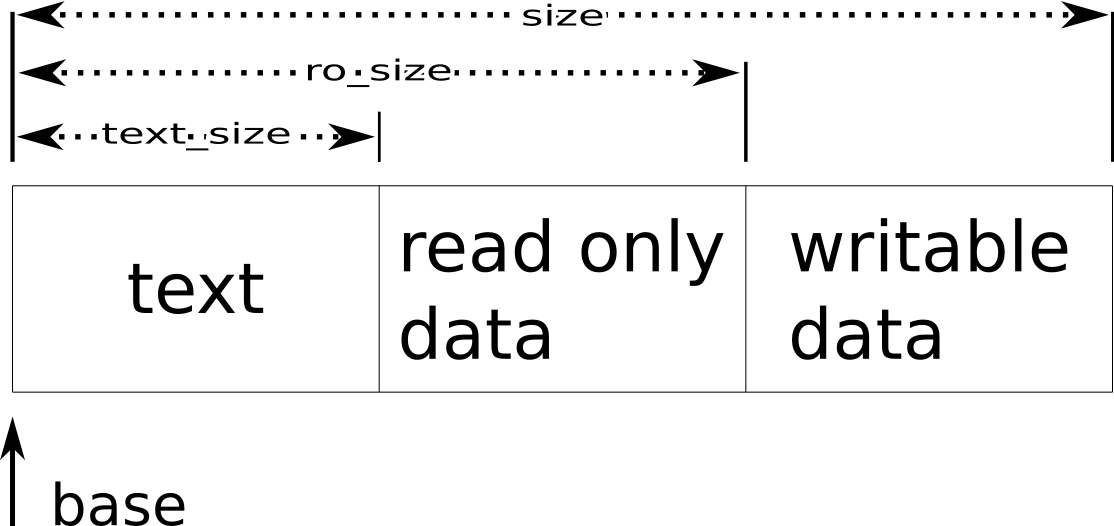
\includegraphics[width=0.75\textwidth]{module-binary_svg}
\caption{Module binary layout in physical memory (figure labels same as the variable names in \textit{struct module\_layout}) \label{fig:binaryLayout1}}
\end{figure}

There are two memory regions created in that format, when a module is being installed. These are called \textit{init\_layout} and \textit{core\_layout}. The former region contains all the functions in the module's source code which are have  \textit{\_\_init} attribute added to them. This attribute is used to identify the part of module which only gets used during modules initialization, i.e. when its \textit{init}\footnote{defined with module\_init() macro} function gets executed. After that this area is freed. \textit{core\_layout} lives throughout the life of the module, and only gets freed when module is removed.
\\\\
The code generated by \textit{gcc} for modules is in such a way that favours relocation. Firstly, gcc tries to use relative references in code (relative jump statements, etc.) making relocations easier. Secondly, every section of module binary that needs relocation has an associated relocation section which helps in relocation of code of that particular section.

\item \textbf{Interrupt remapping}\\
To avoid involvement of host during processing of interrupt from a device, it is better to map it to the isolated space directly. For this the machine must support VT-d, with IOMMU, and interrupt remapping. The CPU may not support interrupt remapping even if it supports VT-d. To check if it does, do the following\footnote{http://www.linux-kvm.org/page/How\_to\_assign\_devices\_with\_VT-d\_in\_KVM}(intel CPU).

\begin{lstlisting}
dmesg | grep -i -e DMAR -e IOMMU
[    0.000000] ACPI: DMAR 0x00000000DBB29CD0 0000B8 (v01 INTEL  DB85FL   00000082 INTL 00000001)
[    0.022778] DMAR: Host address width 39
[    0.022780] DMAR: DRHD base: 0x000000fed90000 flags: 0x0
[    0.022786] DMAR: dmar0: reg_base_addr fed90000 ver 1:0 cap c0000020660462 ecap f0101a
[    0.022787] DMAR: DRHD base: 0x000000fed91000 flags: 0x1
[    0.022789] DMAR: dmar1: reg_base_addr fed91000 ver 1:0 cap d2008020660462 ecap f010da
[    0.022790] DMAR: RMRR base: 0x000000dbeba000 end: 0x000000dbec8fff
[    0.022791] DMAR: RMRR base: 0x000000dd000000 end: 0x000000df1fffff
[    0.022793] DMAR-IR: IOAPIC id 8 under DRHD base  0xfed91000 IOMMU 1
[    0.022794] DMAR-IR: HPET id 0 under DRHD base 0xfed91000
[    0.022795] DMAR-IR: Queued invalidation will be enabled to support x2apic and Intr-remapping.
[    0.023057] DMAR-IR: Enabled IRQ remapping in x2apic mode

\end{lstlisting}

\item \textbf{Passthrough}\\
Passthrough enables a device to be enabled to a VM exclusively. The VM can use the device without involving the host. This cannot be done with all devices. It also depends on the support provided by hypervisor. KVM for example as of now doesn't support doing a passthrough of the GPU.
\item \textbf{Communication with user space component}\\
As discussed previously kernel space component of the user space driver exposed some special files so that the user space component can \textit{mmap} the memory of device, and know about the interrupts. Now since in our case the kernel module runs in isolated space, a mechanism should be set up to allow to-and-fro communication between these two parts of the driver.
\item \textbf{Memory management}\\
During the course of its execution the kernel module will have to allocate and free memory several times. Since, the kernel module is running in an isolated space, these mechanisms must be provided to it explicitly. KVM doesn't allow guest memory to grow and shrink dynamically, thus some memory may have to reserved in advance to satisfy memory requirements of the module.
\item \textbf{Driver and interrupt handler registration}\\
When the module will run its \textit{init} function, it will try to register itself as a driver for a particular set of devices, so that when the device gets attached the kernel notifies the module by calling its probe function.\\\\
This work as of now only creates a minimal environment in isolated space, because of which the features like communication with user space, passthrough, interrupt remapping, driver and interrupt handler registration, and memory management are not supported. Some very basic modules are only able to run in the isolated space as of now. To provide complete support for user space drivers, these missing components need to be implemented as well.
\end{enumerate}



\chapter{Tests and Experimentation}
%\chapter{Verification of correctness}
\chapter{Future work}
\begin{enumerate}
\item \textbf{Testing on real H/W}\\
The components of the project have been tested individually, but a test using real hardware needs to be done. Finding a hardware which uses user space drivers, without using UIO core, and is easily available is a challenge.

\item \textbf{UIO core}\\
The UIO core provided by Linux kernel simplifies the development of user space drivers to a great extent. Providing its support in the isolated space we create would enable UIO drivers to be supported right away. Increasing the variety of drivers that can be supported. 

\item \textbf{Shared interrupts and device multiplexing}\\
The proposed system does not support shared interrupts, it also requires 1-1 correspondence between a device and the container using it. Future versions may provide support for shared interrupts, and multiplexing of devices between several containers.

\item \textbf{Mainlining}\\
If the code of this project can be merged with the mainline LXC repository then that will establish its significance.

\item \textbf{Supporting systems without virtualization extensions}\\
To figure out if the proposed mechanism can be ported to systems which do no have support for virtualization extensions (like older x86 processors) we have used. Some amount of binary patching may be required.

\item \textbf{Study coupling of other classes of kernel modules with kernel-call graphs}\\
Right now we have only explored user space drivers, there may be other classes of drivers in the kernel which share the characteristics of user space drivers of having low coupling with the kernel. Later on a mechanism to support devices with high coupling can also be studied.

\item \textbf{Other applications of the isolated space}\\
Finding other areas of software development which can benefit from creating such an isolated space using virtualization extensions.

\end{enumerate}

\chapter{Conclusion}
User space drivers form an important class of drivers in the Linux kernel.
A mechanism to support use of user space drivers was proposed and partially implemented. The system in its current state supports installation of simple kernel modules from containers without compromising other containers. To fully provide support for user space drivers all the proposed components(chapter~\ref{ch:implementation}) have to be implemented.
\nocite{*}
\bibliographystyle{plain}
\bibliography{biblio}
\end{document}
complete-
Isolated space creation
may include-
\section{Salient features}
\section{Analysis of a kernel module binary}
\subsection{Sections and symbols}